\documentclass[1p]{elsarticle_modified}
%\bibliographystyle{elsarticle-num}

%\usepackage[colorlinks]{hyperref}
%\usepackage{abbrmath_seonhwa} %\Abb, \Ascr, \Acal ,\Abf, \Afrak
\usepackage{amsfonts}
\usepackage{amssymb}
\usepackage{amsmath}
\usepackage{amsthm}
\usepackage{scalefnt}
\usepackage{amsbsy}
\usepackage{kotex}
\usepackage{caption}
\usepackage{subfig}
\usepackage{color}
\usepackage{graphicx}
\usepackage{xcolor} %% white, black, red, green, blue, cyan, magenta, yellow
\usepackage{float}
\usepackage{setspace}
\usepackage{hyperref}

\usepackage{tikz}
\usetikzlibrary{arrows}

\usepackage{multirow}
\usepackage{array} % fixed length table
\usepackage{hhline}

%%%%%%%%%%%%%%%%%%%%%
\makeatletter
\renewcommand*\env@matrix[1][\arraystretch]{%
	\edef\arraystretch{#1}%
	\hskip -\arraycolsep
	\let\@ifnextchar\new@ifnextchar
	\array{*\c@MaxMatrixCols c}}
\makeatother %https://tex.stackexchange.com/questions/14071/how-can-i-increase-the-line-spacing-in-a-matrix
%%%%%%%%%%%%%%%

\usepackage[normalem]{ulem}

\newcommand{\msout}[1]{\ifmmode\text{\sout{\ensuremath{#1}}}\else\sout{#1}\fi}
%SOURCE: \msout is \stkout macro in https://tex.stackexchange.com/questions/20609/strikeout-in-math-mode

\newcommand{\cancel}[1]{
	\ifmmode
	{\color{red}\msout{#1}}
	\else
	{\color{red}\sout{#1}}
	\fi
}

\newcommand{\add}[1]{
	{\color{blue}\uwave{#1}}
}

\newcommand{\replace}[2]{
	\ifmmode
	{\color{red}\msout{#1}}{\color{blue}\uwave{#2}}
	\else
	{\color{red}\sout{#1}}{\color{blue}\uwave{#2}}
	\fi
}

\newcommand{\Sol}{\mathcal{S}} %segment
\newcommand{\D}{D} %diagram
\newcommand{\A}{\mathcal{A}} %arc


%%%%%%%%%%%%%%%%%%%%%%%%%%%%%5 test

\def\sl{\operatorname{\textup{SL}}(2,\Cbb)}
\def\psl{\operatorname{\textup{PSL}}(2,\Cbb)}
\def\quan{\mkern 1mu \triangleright \mkern 1mu}

\theoremstyle{definition}
\newtheorem{thm}{Theorem}[section]
\newtheorem{prop}[thm]{Proposition}
\newtheorem{lem}[thm]{Lemma}
\newtheorem{ques}[thm]{Question}
\newtheorem{cor}[thm]{Corollary}
\newtheorem{defn}[thm]{Definition}
\newtheorem{exam}[thm]{Example}
\newtheorem{rmk}[thm]{Remark}
\newtheorem{alg}[thm]{Algorithm}

\newcommand{\I}{\sqrt{-1}}
\begin{document}

%\begin{frontmatter}
%
%\title{Boundary parabolic representations of knots up to 8 crossings}
%
%%% Group authors per affiliation:
%\author{Yunhi Cho} 
%\address{Department of Mathematics, University of Seoul, Seoul, Korea}
%\ead{yhcho@uos.ac.kr}
%
%
%\author{Seonhwa Kim} %\fnref{s_kim}}
%\address{Center for Geometry and Physics, Institute for Basic Science, Pohang, 37673, Korea}
%\ead{ryeona17@ibs.re.kr}
%
%\author{Hyuk Kim}
%\address{Department of Mathematical Sciences, Seoul National University, Seoul 08826, Korea}
%\ead{hyukkim@snu.ac.kr}
%
%\author{Seokbeom Yoon}
%\address{Department of Mathematical Sciences, Seoul National University, Seoul, 08826,  Korea}
%\ead{sbyoon15@snu.ac.kr}
%
%\begin{abstract}
%We find all boundary parabolic representation of knots up to 8 crossings.
%
%\end{abstract}
%\begin{keyword}
%    \MSC[2010] 57M25 
%\end{keyword}
%
%\end{frontmatter}

%\linenumbers
%\tableofcontents
%
\newcommand\colored[1]{\textcolor{white}{\rule[-0.35ex]{0.8em}{1.4ex}}\kern-0.8em\color{red} #1}%
%\newcommand\colored[1]{\textcolor{white}{ #1}\kern-2.17ex	\textcolor{white}{ #1}\kern-1.81ex	\textcolor{white}{ #1}\kern-2.15ex\color{red}#1	}

{\Large $\underline{12a_{0930}~(K12a_{0930})}$}

\setlength{\tabcolsep}{10pt}
\renewcommand{\arraystretch}{1.6}
\vspace{1cm}\begin{tabular}{m{100pt}>{\centering\arraybackslash}m{274pt}}
\multirow{5}{120pt}{
	\centering
	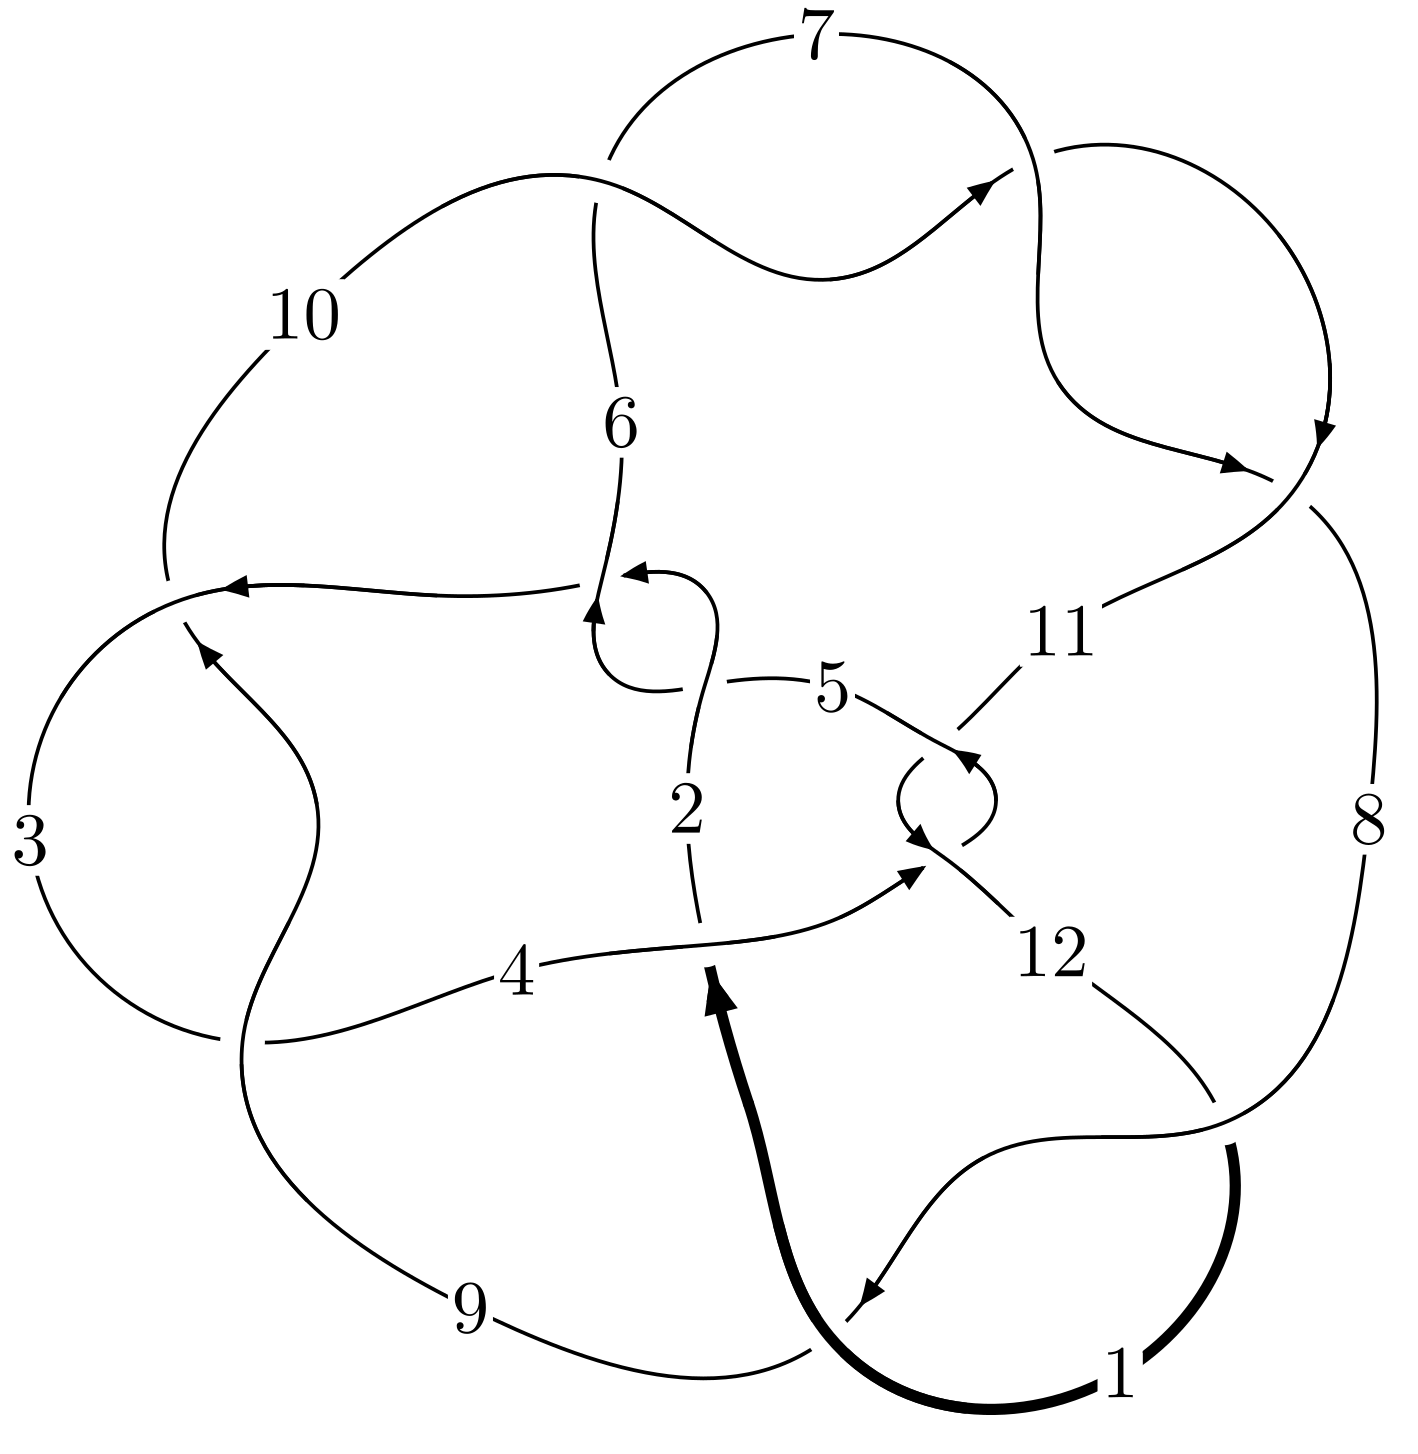
\includegraphics[width=112pt]{../../../GIT/diagram.site/Diagrams/png/1731_12a_0930.png}\\
\ \ \ A knot diagram\footnotemark}&
\allowdisplaybreaks
\textbf{Linearized knot diagam} \\
\cline{2-2}
 &
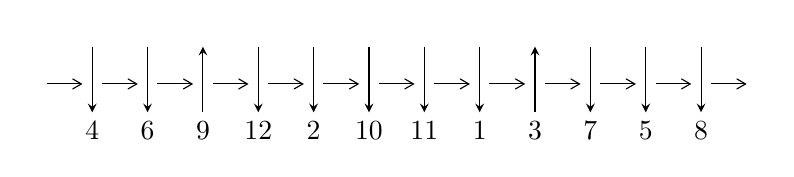
\begin{tikzpicture}[x=20pt, y=17pt]
	% nodes
	\node (C0) at (0, 0) {};
	\node (C1) at (1, 0) {};
	\node (C1U) at (1, +1) {};
	\node (C1D) at (1, -1) {4};

	\node (C2) at (2, 0) {};
	\node (C2U) at (2, +1) {};
	\node (C2D) at (2, -1) {6};

	\node (C3) at (3, 0) {};
	\node (C3U) at (3, +1) {};
	\node (C3D) at (3, -1) {9};

	\node (C4) at (4, 0) {};
	\node (C4U) at (4, +1) {};
	\node (C4D) at (4, -1) {12};

	\node (C5) at (5, 0) {};
	\node (C5U) at (5, +1) {};
	\node (C5D) at (5, -1) {2};

	\node (C6) at (6, 0) {};
	\node (C6U) at (6, +1) {};
	\node (C6D) at (6, -1) {10};

	\node (C7) at (7, 0) {};
	\node (C7U) at (7, +1) {};
	\node (C7D) at (7, -1) {11};

	\node (C8) at (8, 0) {};
	\node (C8U) at (8, +1) {};
	\node (C8D) at (8, -1) {1};

	\node (C9) at (9, 0) {};
	\node (C9U) at (9, +1) {};
	\node (C9D) at (9, -1) {3};

	\node (C10) at (10, 0) {};
	\node (C10U) at (10, +1) {};
	\node (C10D) at (10, -1) {7};

	\node (C11) at (11, 0) {};
	\node (C11U) at (11, +1) {};
	\node (C11D) at (11, -1) {5};

	\node (C12) at (12, 0) {};
	\node (C12U) at (12, +1) {};
	\node (C12D) at (12, -1) {8};
	\node (C13) at (13, 0) {};

	% arrows
	\draw[->,>={angle 60}]
	(C0) edge (C1) (C1) edge (C2) (C2) edge (C3) (C3) edge (C4) (C4) edge (C5) (C5) edge (C6) (C6) edge (C7) (C7) edge (C8) (C8) edge (C9) (C9) edge (C10) (C10) edge (C11) (C11) edge (C12) (C12) edge (C13) ;	\draw[->,>=stealth]
	(C1U) edge (C1D) (C2U) edge (C2D) (C3D) edge (C3U) (C4U) edge (C4D) (C5U) edge (C5D) (C6U) edge (C6D) (C7U) edge (C7D) (C8U) edge (C8D) (C9D) edge (C9U) (C10U) edge (C10D) (C11U) edge (C11D) (C12U) edge (C12D) ;
	\end{tikzpicture} \\
\hhline{~~} \\& 
\textbf{Solving Sequence} \\ \cline{2-2} 
 &
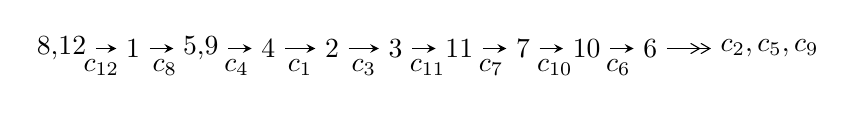
\begin{tikzpicture}[x=23pt, y=7pt]
	% node
	\node (A0) at (-1/8, 0) {8,12};
	\node (A1) at (1, 0) {1};
	\node (A2) at (33/16, 0) {5,9};
	\node (A3) at (25/8, 0) {4};
	\node (A4) at (33/8, 0) {2};
	\node (A5) at (41/8, 0) {3};
	\node (A6) at (49/8, 0) {11};
	\node (A7) at (57/8, 0) {7};
	\node (A8) at (65/8, 0) {10};
	\node (A9) at (73/8, 0) {6};
	\node (C1) at (1/2, -1) {$c_{12}$};
	\node (C2) at (3/2, -1) {$c_{8}$};
	\node (C3) at (21/8, -1) {$c_{4}$};
	\node (C4) at (29/8, -1) {$c_{1}$};
	\node (C5) at (37/8, -1) {$c_{3}$};
	\node (C6) at (45/8, -1) {$c_{11}$};
	\node (C7) at (53/8, -1) {$c_{7}$};
	\node (C8) at (61/8, -1) {$c_{10}$};
	\node (C9) at (69/8, -1) {$c_{6}$};
	\node (A10) at (11, 0) {$c_{2},c_{5},c_{9}$};

	% edge
	\draw[->,>=stealth]	
	(A0) edge (A1) (A1) edge (A2) (A2) edge (A3) (A3) edge (A4) (A4) edge (A5) (A5) edge (A6) (A6) edge (A7) (A7) edge (A8) (A8) edge (A9) ;
	\draw[->>,>={angle 60}]	
	(A9) edge (A10);
\end{tikzpicture} \\ 

\end{tabular} \\

\footnotetext{
The image of knot diagram is generated by the software ``\textbf{Draw programme}" developed by Andrew Bartholomew(\url{http://www.layer8.co.uk/maths/draw/index.htm\#Running-draw}), where we modified some parts for our purpose(\url{https://github.com/CATsTAILs/LinksPainter}).
}\phantom \\ \newline 
\centering \textbf{Ideals for irreducible components\footnotemark of $X_{\text{par}}$} 
 
\begin{align*}
I^u_{1}&=\langle 
9.59690\times10^{335} u^{96}-1.05215\times10^{336} u^{95}+\cdots+3.44266\times10^{336} b-5.12396\times10^{337},\\
\phantom{I^u_{1}}&\phantom{= \langle  }8.78993\times10^{338} u^{96}-1.24791\times10^{339} u^{95}+\cdots+3.52873\times10^{339} a+1.10173\times10^{340},\\
\phantom{I^u_{1}}&\phantom{= \langle  }u^{97}-2 u^{96}+\cdots+1714 u+41\rangle \\
I^u_{2}&=\langle 
509208711230210 u^{22}+109407337183821 u^{21}+\cdots+56843194846091 b+2350612385286411,\\
\phantom{I^u_{2}}&\phantom{= \langle  }-7.80907\times10^{15} u^{22}-1.63603\times10^{15} u^{21}+\cdots+2.84216\times10^{14} a-3.68176\times10^{16},\;u^{23}-7 u^{21}+\cdots+8 u-1\rangle \\
I^u_{3}&=\langle 
b+1,\;a+1,\;u+1\rangle \\
\\
\end{align*}
\raggedright * 3 irreducible components of $\dim_{\mathbb{C}}=0$, with total 121 representations.\\
\footnotetext{All coefficients of polynomials are rational numbers. But the coefficients are sometimes approximated in decimal forms when there is not enough margin.}
\newpage
\renewcommand{\arraystretch}{1}
\centering \section*{I. $I^u_{1}= \langle 9.60\times10^{335} u^{96}-1.05\times10^{336} u^{95}+\cdots+3.44\times10^{336} b-5.12\times10^{337},\;8.79\times10^{338} u^{96}-1.25\times10^{339} u^{95}+\cdots+3.53\times10^{339} a+1.10\times10^{340},\;u^{97}-2 u^{96}+\cdots+1714 u+41 \rangle$}
\flushleft \textbf{(i) Arc colorings}\\
\begin{tabular}{m{7pt} m{180pt} m{7pt} m{180pt} }
\flushright $a_{8}=$&$\begin{pmatrix}0\\u\end{pmatrix}$ \\
\flushright $a_{12}=$&$\begin{pmatrix}1\\0\end{pmatrix}$ \\
\flushright $a_{1}=$&$\begin{pmatrix}1\\u^2\end{pmatrix}$ \\
\flushright $a_{5}=$&$\begin{pmatrix}-0.249096 u^{96}+0.353643 u^{95}+\cdots+791.383 u-3.12216\\-0.278764 u^{96}+0.305620 u^{95}+\cdots+673.123 u+14.8837\end{pmatrix}$ \\
\flushright $a_{9}=$&$\begin{pmatrix}- u\\- u^3+u\end{pmatrix}$ \\
\flushright $a_{4}=$&$\begin{pmatrix}-0.527860 u^{96}+0.659263 u^{95}+\cdots+1464.51 u+11.7615\\-0.278764 u^{96}+0.305620 u^{95}+\cdots+673.123 u+14.8837\end{pmatrix}$ \\
\flushright $a_{2}=$&$\begin{pmatrix}-0.0762388 u^{96}-0.0826739 u^{95}+\cdots-282.307 u+8.80990\\0.140133 u^{96}-0.171057 u^{95}+\cdots-376.086 u-8.22131\end{pmatrix}$ \\
\flushright $a_{3}=$&$\begin{pmatrix}-0.340979 u^{96}+0.446598 u^{95}+\cdots+974.929 u+0.494949\\-0.323338 u^{96}+0.384426 u^{95}+\cdots+878.917 u+19.5453\end{pmatrix}$ \\
\flushright $a_{11}=$&$\begin{pmatrix}0.0726071 u^{96}-0.0690112 u^{95}+\cdots-167.910 u-16.7409\\0.199514 u^{96}-0.0750754 u^{95}+\cdots-320.938 u-8.18508\end{pmatrix}$ \\
\flushright $a_{7}=$&$\begin{pmatrix}-0.0146069 u^{96}-0.0282631 u^{95}+\cdots-99.5227 u-6.12905\\-0.699903 u^{96}+0.763490 u^{95}+\cdots+1488.36 u+34.3576\end{pmatrix}$ \\
\flushright $a_{10}=$&$\begin{pmatrix}-0.366501 u^{96}+0.396659 u^{95}+\cdots+785.732 u+6.52821\\-0.343656 u^{96}+0.391918 u^{95}+\cdots+332.980 u+7.46440\end{pmatrix}$ \\
\flushright $a_{6}=$&$\begin{pmatrix}0.204866 u^{96}-0.0714659 u^{95}+\cdots-29.8300 u-8.45377\\-0.0464229 u^{96}+0.0479177 u^{95}+\cdots+147.679 u+3.12461\end{pmatrix}$\\&\end{tabular}
\flushleft \textbf{(ii) Obstruction class $= -1$}\\~\\
\flushleft \textbf{(iii) Cusp Shapes $= -1.92098 u^{96}+3.83799 u^{95}+\cdots-1343.96 u-38.2137$}\\~\\
\newpage\renewcommand{\arraystretch}{1}
\flushleft \textbf{(iv) u-Polynomials at the component}\newline \\
\begin{tabular}{m{50pt}|m{274pt}}
Crossings & \hspace{64pt}u-Polynomials at each crossing \\
\hline $$\begin{aligned}c_{1}\end{aligned}$$&$\begin{aligned}
&u^{97}-13 u^{96}+\cdots+83802 u-29149
\end{aligned}$\\
\hline $$\begin{aligned}c_{2},c_{5}\end{aligned}$$&$\begin{aligned}
&u^{97}- u^{96}+\cdots-22184 u-2161
\end{aligned}$\\
\hline $$\begin{aligned}c_{3},c_{9}\end{aligned}$$&$\begin{aligned}
&u^{97}-14 u^{96}+\cdots+1812 u-149
\end{aligned}$\\
\hline $$\begin{aligned}c_{4},c_{11}\end{aligned}$$&$\begin{aligned}
&u^{97}-3 u^{96}+\cdots-356 u-59
\end{aligned}$\\
\hline $$\begin{aligned}c_{6},c_{7},c_{10}\end{aligned}$$&$\begin{aligned}
&u^{97}+4 u^{96}+\cdots+4242 u+242
\end{aligned}$\\
\hline $$\begin{aligned}c_{8},c_{12}\end{aligned}$$&$\begin{aligned}
&u^{97}-2 u^{96}+\cdots+1714 u+41
\end{aligned}$\\
\hline
\end{tabular}\\~\\
\newpage\renewcommand{\arraystretch}{1}
\flushleft \textbf{(v) Riley Polynomials at the component}\newline \\
\begin{tabular}{m{50pt}|m{274pt}}
Crossings & \hspace{64pt}Riley Polynomials at each crossing \\
\hline $$\begin{aligned}c_{1}\end{aligned}$$&$\begin{aligned}
&y^{97}-37 y^{96}+\cdots+128682539484 y-849664201
\end{aligned}$\\
\hline $$\begin{aligned}c_{2},c_{5}\end{aligned}$$&$\begin{aligned}
&y^{97}-79 y^{96}+\cdots+423448954 y-4669921
\end{aligned}$\\
\hline $$\begin{aligned}c_{3},c_{9}\end{aligned}$$&$\begin{aligned}
&y^{97}-3452 y^{95}+\cdots-696744 y-22201
\end{aligned}$\\
\hline $$\begin{aligned}c_{4},c_{11}\end{aligned}$$&$\begin{aligned}
&y^{97}-47 y^{96}+\cdots-64542 y-3481
\end{aligned}$\\
\hline $$\begin{aligned}c_{6},c_{7},c_{10}\end{aligned}$$&$\begin{aligned}
&y^{97}-110 y^{96}+\cdots+17376496 y-58564
\end{aligned}$\\
\hline $$\begin{aligned}c_{8},c_{12}\end{aligned}$$&$\begin{aligned}
&y^{97}-68 y^{96}+\cdots+2983388 y-1681
\end{aligned}$\\
\hline
\end{tabular}\\~\\
\newpage\flushleft \textbf{(vi) Complex Volumes and Cusp Shapes}
$$\begin{array}{c|c|c}  
\text{Solutions to }I^u_{1}& \I (\text{vol} + \sqrt{-1}CS) & \text{Cusp shape}\\
 \hline 
\begin{aligned}
u &= -1.00099\phantom{ +0.000000I} \\
a &= \phantom{-}0.104557\phantom{ +0.000000I} \\
b &= \phantom{-}8.97759\phantom{ +0.000000I}\end{aligned}
 & -3.28781\phantom{ +0.000000I} & -2205.50\phantom{ +0.000000I} \\ \hline\begin{aligned}
u &= -0.236628 + 0.987183 I \\
a &= \phantom{-}0.733045 + 1.115450 I \\
b &= -0.640466 - 1.082220 I\end{aligned}
 & -5.18696 - 5.17546 I & \phantom{-0.000000 } 0 \\ \hline\begin{aligned}
u &= -0.236628 - 0.987183 I \\
a &= \phantom{-}0.733045 - 1.115450 I \\
b &= -0.640466 + 1.082220 I\end{aligned}
 & -5.18696 + 5.17546 I & \phantom{-0.000000 } 0 \\ \hline\begin{aligned}
u &= \phantom{-}1.006690 + 0.203483 I \\
a &= \phantom{-}1.35334 - 1.08695 I \\
b &= \phantom{-}0.454354 + 0.669034 I\end{aligned}
 & -3.28245 - 0.83839 I & \phantom{-0.000000 } 0 \\ \hline\begin{aligned}
u &= \phantom{-}1.006690 - 0.203483 I \\
a &= \phantom{-}1.35334 + 1.08695 I \\
b &= \phantom{-}0.454354 - 0.669034 I\end{aligned}
 & -3.28245 + 0.83839 I & \phantom{-0.000000 } 0 \\ \hline\begin{aligned}
u &= \phantom{-}0.059389 + 1.035400 I \\
a &= \phantom{-}0.00927 - 1.53980 I \\
b &= \phantom{-}0.430082 + 1.145650 I\end{aligned}
 & -2.87174 - 6.62403 I & \phantom{-0.000000 } 0 \\ \hline\begin{aligned}
u &= \phantom{-}0.059389 - 1.035400 I \\
a &= \phantom{-}0.00927 + 1.53980 I \\
b &= \phantom{-}0.430082 - 1.145650 I\end{aligned}
 & -2.87174 + 6.62403 I & \phantom{-0.000000 } 0 \\ \hline\begin{aligned}
u &= -1.041690 + 0.037723 I \\
a &= \phantom{-}0.863323 - 0.623359 I \\
b &= \phantom{-}0.534994 + 1.031760 I\end{aligned}
 & -2.20470 + 0.29278 I & \phantom{-0.000000 } 0 \\ \hline\begin{aligned}
u &= -1.041690 - 0.037723 I \\
a &= \phantom{-}0.863323 + 0.623359 I \\
b &= \phantom{-}0.534994 - 1.031760 I\end{aligned}
 & -2.20470 - 0.29278 I & \phantom{-0.000000 } 0 \\ \hline\begin{aligned}
u &= -0.987860 + 0.352019 I \\
a &= -0.934926 - 0.230856 I \\
b &= -0.173771 + 0.697387 I\end{aligned}
 & -0.897884 - 0.166548 I & \phantom{-0.000000 } 0\\
 \hline 
 \end{array}$$\newpage$$\begin{array}{c|c|c}  
\text{Solutions to }I^u_{1}& \I (\text{vol} + \sqrt{-1}CS) & \text{Cusp shape}\\
 \hline 
\begin{aligned}
u &= -0.987860 - 0.352019 I \\
a &= -0.934926 + 0.230856 I \\
b &= -0.173771 - 0.697387 I\end{aligned}
 & -0.897884 + 0.166548 I & \phantom{-0.000000 } 0 \\ \hline\begin{aligned}
u &= \phantom{-}0.937667\phantom{ +0.000000I} \\
a &= -0.678354\phantom{ +0.000000I} \\
b &= -3.75942\phantom{ +0.000000I}\end{aligned}
 & -8.62239\phantom{ +0.000000I} & \phantom{-0.000000 } 0 \\ \hline\begin{aligned}
u &= \phantom{-}0.543866 + 0.923125 I \\
a &= -0.82668 + 1.28337 I \\
b &= \phantom{-}0.571458 - 0.472121 I\end{aligned}
 & -12.51620 - 5.63081 I & \phantom{-0.000000 } 0 \\ \hline\begin{aligned}
u &= \phantom{-}0.543866 - 0.923125 I \\
a &= -0.82668 - 1.28337 I \\
b &= \phantom{-}0.571458 + 0.472121 I\end{aligned}
 & -12.51620 + 5.63081 I & \phantom{-0.000000 } 0 \\ \hline\begin{aligned}
u &= -0.403795 + 0.996611 I \\
a &= -0.79352 - 1.17354 I \\
b &= \phantom{-}0.418677 + 0.887734 I\end{aligned}
 & -1.17057 - 1.72797 I & \phantom{-0.000000 } 0 \\ \hline\begin{aligned}
u &= -0.403795 - 0.996611 I \\
a &= -0.79352 + 1.17354 I \\
b &= \phantom{-}0.418677 - 0.887734 I\end{aligned}
 & -1.17057 + 1.72797 I & \phantom{-0.000000 } 0 \\ \hline\begin{aligned}
u &= -1.089510 + 0.121285 I \\
a &= -1.83583 + 0.43767 I \\
b &= -0.415865 - 0.714017 I\end{aligned}
 & -7.90895 + 0.71724 I & \phantom{-0.000000 } 0 \\ \hline\begin{aligned}
u &= -1.089510 - 0.121285 I \\
a &= -1.83583 - 0.43767 I \\
b &= -0.415865 + 0.714017 I\end{aligned}
 & -7.90895 - 0.71724 I & \phantom{-0.000000 } 0 \\ \hline\begin{aligned}
u &= \phantom{-}1.115620 + 0.034953 I \\
a &= \phantom{-}0.492249 - 1.264290 I \\
b &= \phantom{-}0.55813 + 1.63026 I\end{aligned}
 & -7.70818 - 2.22028 I & \phantom{-0.000000 } 0 \\ \hline\begin{aligned}
u &= \phantom{-}1.115620 - 0.034953 I \\
a &= \phantom{-}0.492249 + 1.264290 I \\
b &= \phantom{-}0.55813 - 1.63026 I\end{aligned}
 & -7.70818 + 2.22028 I & \phantom{-0.000000 } 0\\
 \hline 
 \end{array}$$\newpage$$\begin{array}{c|c|c}  
\text{Solutions to }I^u_{1}& \I (\text{vol} + \sqrt{-1}CS) & \text{Cusp shape}\\
 \hline 
\begin{aligned}
u &= \phantom{-}0.359991 + 0.802181 I \\
a &= -0.296638 + 1.381910 I \\
b &= \phantom{-}0.062718 - 1.088860 I\end{aligned}
 & \phantom{-}3.34481 - 0.89059 I & \phantom{-0.000000 } 0 \\ \hline\begin{aligned}
u &= \phantom{-}0.359991 - 0.802181 I \\
a &= -0.296638 - 1.381910 I \\
b &= \phantom{-}0.062718 + 1.088860 I\end{aligned}
 & \phantom{-}3.34481 + 0.89059 I & \phantom{-0.000000 } 0 \\ \hline\begin{aligned}
u &= \phantom{-}1.160300 + 0.029718 I \\
a &= -1.14308 + 1.74240 I \\
b &= -0.492514 - 1.084760 I\end{aligned}
 & -14.1423 - 5.8216 I & \phantom{-0.000000 } 0 \\ \hline\begin{aligned}
u &= \phantom{-}1.160300 - 0.029718 I \\
a &= -1.14308 - 1.74240 I \\
b &= -0.492514 + 1.084760 I\end{aligned}
 & -14.1423 + 5.8216 I & \phantom{-0.000000 } 0 \\ \hline\begin{aligned}
u &= \phantom{-}1.108780 + 0.425877 I \\
a &= -0.872737 + 0.916234 I \\
b &= -0.490789 - 1.054630 I\end{aligned}
 & \phantom{-}0.97153 - 3.65106 I & \phantom{-0.000000 } 0 \\ \hline\begin{aligned}
u &= \phantom{-}1.108780 - 0.425877 I \\
a &= -0.872737 - 0.916234 I \\
b &= -0.490789 + 1.054630 I\end{aligned}
 & \phantom{-}0.97153 + 3.65106 I & \phantom{-0.000000 } 0 \\ \hline\begin{aligned}
u &= \phantom{-}1.18971\phantom{ +0.000000I} \\
a &= \phantom{-}0.0975768\phantom{ +0.000000I} \\
b &= -1.62408\phantom{ +0.000000I}\end{aligned}
 & -7.17810\phantom{ +0.000000I} & \phantom{-0.000000 } 0 \\ \hline\begin{aligned}
u &= -0.790199\phantom{ +0.000000I} \\
a &= -0.687237\phantom{ +0.000000I} \\
b &= -0.309181\phantom{ +0.000000I}\end{aligned}
 & -1.20435\phantom{ +0.000000I} & -8.00000\phantom{ +0.000000I} \\ \hline\begin{aligned}
u &= \phantom{-}0.260780 + 0.729992 I \\
a &= -0.81245 - 1.69234 I \\
b &= \phantom{-}0.106403 + 0.939014 I\end{aligned}
 & \phantom{-}0.031297 - 0.283167 I & -10.47064 + 0. I\phantom{ +0.000000I} \\ \hline\begin{aligned}
u &= \phantom{-}0.260780 - 0.729992 I \\
a &= -0.81245 + 1.69234 I \\
b &= \phantom{-}0.106403 - 0.939014 I\end{aligned}
 & \phantom{-}0.031297 + 0.283167 I & -10.47064 + 0. I\phantom{ +0.000000I}\\
 \hline 
 \end{array}$$\newpage$$\begin{array}{c|c|c}  
\text{Solutions to }I^u_{1}& \I (\text{vol} + \sqrt{-1}CS) & \text{Cusp shape}\\
 \hline 
\begin{aligned}
u &= -1.157150 + 0.429543 I \\
a &= \phantom{-}0.58879 + 1.77745 I \\
b &= \phantom{-}0.524055 - 1.081700 I\end{aligned}
 & -9.59278 + 3.62722 I & \phantom{-0.000000 } 0 \\ \hline\begin{aligned}
u &= -1.157150 - 0.429543 I \\
a &= \phantom{-}0.58879 - 1.77745 I \\
b &= \phantom{-}0.524055 + 1.081700 I\end{aligned}
 & -9.59278 - 3.62722 I & \phantom{-0.000000 } 0 \\ \hline\begin{aligned}
u &= -0.160568 + 0.737142 I \\
a &= -0.164412 - 0.618806 I \\
b &= \phantom{-}0.730298 + 0.089390 I\end{aligned}
 & -5.97152 + 2.38544 I & -14.0737 - 2.8213 I \\ \hline\begin{aligned}
u &= -0.160568 - 0.737142 I \\
a &= -0.164412 + 0.618806 I \\
b &= \phantom{-}0.730298 - 0.089390 I\end{aligned}
 & -5.97152 - 2.38544 I & -14.0737 + 2.8213 I \\ \hline\begin{aligned}
u &= \phantom{-}1.228540 + 0.266915 I \\
a &= \phantom{-}0.391803 + 0.241594 I \\
b &= \phantom{-}0.562530 - 0.408648 I\end{aligned}
 & -4.71575 - 3.09828 I & \phantom{-0.000000 } 0 \\ \hline\begin{aligned}
u &= \phantom{-}1.228540 - 0.266915 I \\
a &= \phantom{-}0.391803 - 0.241594 I \\
b &= \phantom{-}0.562530 + 0.408648 I\end{aligned}
 & -4.71575 + 3.09828 I & \phantom{-0.000000 } 0 \\ \hline\begin{aligned}
u &= -1.267880 + 0.177238 I \\
a &= \phantom{-}0.678839 + 0.142037 I \\
b &= \phantom{-}0.526237 - 0.977461 I\end{aligned}
 & -2.23986 + 3.29378 I & \phantom{-0.000000 } 0 \\ \hline\begin{aligned}
u &= -1.267880 - 0.177238 I \\
a &= \phantom{-}0.678839 - 0.142037 I \\
b &= \phantom{-}0.526237 + 0.977461 I\end{aligned}
 & -2.23986 - 3.29378 I & \phantom{-0.000000 } 0 \\ \hline\begin{aligned}
u &= \phantom{-}1.217560 + 0.402996 I \\
a &= \phantom{-}0.814080 - 0.788075 I \\
b &= \phantom{-}0.736447 + 1.145140 I\end{aligned}
 & -1.56639 - 7.72027 I & \phantom{-0.000000 } 0 \\ \hline\begin{aligned}
u &= \phantom{-}1.217560 - 0.402996 I \\
a &= \phantom{-}0.814080 + 0.788075 I \\
b &= \phantom{-}0.736447 - 1.145140 I\end{aligned}
 & -1.56639 + 7.72027 I & \phantom{-0.000000 } 0\\
 \hline 
 \end{array}$$\newpage$$\begin{array}{c|c|c}  
\text{Solutions to }I^u_{1}& \I (\text{vol} + \sqrt{-1}CS) & \text{Cusp shape}\\
 \hline 
\begin{aligned}
u &= \phantom{-}1.240650 + 0.368915 I \\
a &= \phantom{-}0.191262 - 0.405765 I \\
b &= -0.519677 + 1.078090 I\end{aligned}
 & -6.89673 + 1.47760 I & \phantom{-0.000000 } 0 \\ \hline\begin{aligned}
u &= \phantom{-}1.240650 - 0.368915 I \\
a &= \phantom{-}0.191262 + 0.405765 I \\
b &= -0.519677 - 1.078090 I\end{aligned}
 & -6.89673 - 1.47760 I & \phantom{-0.000000 } 0 \\ \hline\begin{aligned}
u &= \phantom{-}1.259380 + 0.349247 I \\
a &= -0.356452 + 0.242013 I \\
b &= -0.997759 + 0.233167 I\end{aligned}
 & -10.25980 - 6.27168 I & \phantom{-0.000000 } 0 \\ \hline\begin{aligned}
u &= \phantom{-}1.259380 - 0.349247 I \\
a &= -0.356452 - 0.242013 I \\
b &= -0.997759 - 0.233167 I\end{aligned}
 & -10.25980 + 6.27168 I & \phantom{-0.000000 } 0 \\ \hline\begin{aligned}
u &= \phantom{-}0.069586 + 0.678813 I \\
a &= \phantom{-}0.359342 - 1.324650 I \\
b &= -0.334946 + 1.148020 I\end{aligned}
 & \phantom{-}1.89522 + 3.59670 I & -3.22502 - 6.27042 I \\ \hline\begin{aligned}
u &= \phantom{-}0.069586 - 0.678813 I \\
a &= \phantom{-}0.359342 + 1.324650 I \\
b &= -0.334946 - 1.148020 I\end{aligned}
 & \phantom{-}1.89522 - 3.59670 I & -3.22502 + 6.27042 I \\ \hline\begin{aligned}
u &= -1.207750 + 0.537510 I \\
a &= \phantom{-}0.652393 + 1.198970 I \\
b &= \phantom{-}0.96200 - 1.24131 I\end{aligned}
 & -8.23196 + 10.60790 I & \phantom{-0.000000 } 0 \\ \hline\begin{aligned}
u &= -1.207750 - 0.537510 I \\
a &= \phantom{-}0.652393 - 1.198970 I \\
b &= \phantom{-}0.96200 + 1.24131 I\end{aligned}
 & -8.23196 - 10.60790 I & \phantom{-0.000000 } 0 \\ \hline\begin{aligned}
u &= -0.251619 + 1.300430 I \\
a &= \phantom{-}0.087461 + 1.259290 I \\
b &= -0.219236 - 0.872762 I\end{aligned}
 & \phantom{-}1.21797 - 1.00031 I & \phantom{-0.000000 } 0 \\ \hline\begin{aligned}
u &= -0.251619 - 1.300430 I \\
a &= \phantom{-}0.087461 - 1.259290 I \\
b &= -0.219236 + 0.872762 I\end{aligned}
 & \phantom{-}1.21797 + 1.00031 I & \phantom{-0.000000 } 0\\
 \hline 
 \end{array}$$\newpage$$\begin{array}{c|c|c}  
\text{Solutions to }I^u_{1}& \I (\text{vol} + \sqrt{-1}CS) & \text{Cusp shape}\\
 \hline 
\begin{aligned}
u &= -1.225120 + 0.503889 I \\
a &= -0.58912 - 1.29789 I \\
b &= -0.71519 + 1.24236 I\end{aligned}
 & -4.07967 + 7.14680 I & \phantom{-0.000000 } 0 \\ \hline\begin{aligned}
u &= -1.225120 - 0.503889 I \\
a &= -0.58912 + 1.29789 I \\
b &= -0.71519 - 1.24236 I\end{aligned}
 & -4.07967 - 7.14680 I & \phantom{-0.000000 } 0 \\ \hline\begin{aligned}
u &= \phantom{-}0.608427 + 0.287937 I \\
a &= -0.794839 - 0.362171 I \\
b &= \phantom{-}0.77786 - 1.38261 I\end{aligned}
 & -8.53694 - 1.57343 I & -10.60265 + 1.06566 I \\ \hline\begin{aligned}
u &= \phantom{-}0.608427 - 0.287937 I \\
a &= -0.794839 + 0.362171 I \\
b &= \phantom{-}0.77786 + 1.38261 I\end{aligned}
 & -8.53694 + 1.57343 I & -10.60265 - 1.06566 I \\ \hline\begin{aligned}
u &= -0.015635 + 1.347280 I \\
a &= -0.399900 + 1.334910 I \\
b &= \phantom{-}0.584733 - 1.067800 I\end{aligned}
 & -10.7431 + 10.3794 I & \phantom{-0.000000 } 0 \\ \hline\begin{aligned}
u &= -0.015635 - 1.347280 I \\
a &= -0.399900 - 1.334910 I \\
b &= \phantom{-}0.584733 + 1.067800 I\end{aligned}
 & -10.7431 - 10.3794 I & \phantom{-0.000000 } 0 \\ \hline\begin{aligned}
u &= \phantom{-}0.618891 + 0.184854 I \\
a &= -1.80641 + 2.28001 I \\
b &= \phantom{-}0.333765 + 0.342067 I\end{aligned}
 & -12.12580 - 5.94770 I & -17.3706 + 1.5513 I \\ \hline\begin{aligned}
u &= \phantom{-}0.618891 - 0.184854 I \\
a &= -1.80641 - 2.28001 I \\
b &= \phantom{-}0.333765 - 0.342067 I\end{aligned}
 & -12.12580 + 5.94770 I & -17.3706 - 1.5513 I \\ \hline\begin{aligned}
u &= -1.171010 + 0.697628 I \\
a &= -0.456614 - 1.290590 I \\
b &= -0.473878 + 0.657609 I\end{aligned}
 & -8.20157 + 2.65755 I & \phantom{-0.000000 } 0 \\ \hline\begin{aligned}
u &= -1.171010 - 0.697628 I \\
a &= -0.456614 + 1.290590 I \\
b &= -0.473878 - 0.657609 I\end{aligned}
 & -8.20157 - 2.65755 I & \phantom{-0.000000 } 0\\
 \hline 
 \end{array}$$\newpage$$\begin{array}{c|c|c}  
\text{Solutions to }I^u_{1}& \I (\text{vol} + \sqrt{-1}CS) & \text{Cusp shape}\\
 \hline 
\begin{aligned}
u &= \phantom{-}1.314220 + 0.407705 I \\
a &= \phantom{-}0.928702 - 0.304670 I \\
b &= \phantom{-}0.347914 + 0.703563 I\end{aligned}
 & -3.57329 - 3.99154 I & \phantom{-0.000000 } 0 \\ \hline\begin{aligned}
u &= \phantom{-}1.314220 - 0.407705 I \\
a &= \phantom{-}0.928702 + 0.304670 I \\
b &= \phantom{-}0.347914 - 0.703563 I\end{aligned}
 & -3.57329 + 3.99154 I & \phantom{-0.000000 } 0 \\ \hline\begin{aligned}
u &= -0.587686 + 0.184049 I \\
a &= \phantom{-}0.17715 - 1.94184 I \\
b &= -0.143820 + 1.355940 I\end{aligned}
 & \phantom{-}1.24512 + 2.95965 I & -17.1971 - 8.3280 I \\ \hline\begin{aligned}
u &= -0.587686 - 0.184049 I \\
a &= \phantom{-}0.17715 + 1.94184 I \\
b &= -0.143820 - 1.355940 I\end{aligned}
 & \phantom{-}1.24512 - 2.95965 I & -17.1971 + 8.3280 I \\ \hline\begin{aligned}
u &= \phantom{-}1.380920 + 0.295378 I \\
a &= -1.091370 + 0.168749 I \\
b &= -0.484273 - 0.978684 I\end{aligned}
 & -6.97072 - 4.52407 I & \phantom{-0.000000 } 0 \\ \hline\begin{aligned}
u &= \phantom{-}1.380920 - 0.295378 I \\
a &= -1.091370 - 0.168749 I \\
b &= -0.484273 + 0.978684 I\end{aligned}
 & -6.97072 + 4.52407 I & \phantom{-0.000000 } 0 \\ \hline\begin{aligned}
u &= -1.37522 + 0.33577 I \\
a &= \phantom{-}0.1227200 + 0.0495155 I \\
b &= -1.37069 - 0.43293 I\end{aligned}
 & -18.2002 + 9.6383 I & \phantom{-0.000000 } 0 \\ \hline\begin{aligned}
u &= -1.37522 - 0.33577 I \\
a &= \phantom{-}0.1227200 - 0.0495155 I \\
b &= -1.37069 + 0.43293 I\end{aligned}
 & -18.2002 - 9.6383 I & \phantom{-0.000000 } 0 \\ \hline\begin{aligned}
u &= -0.194872 + 0.521399 I \\
a &= \phantom{-}1.36940 + 1.36276 I \\
b &= \phantom{-}0.294275 - 1.219930 I\end{aligned}
 & -2.02000 + 1.29634 I & -8.59011 - 0.82038 I \\ \hline\begin{aligned}
u &= -0.194872 - 0.521399 I \\
a &= \phantom{-}1.36940 - 1.36276 I \\
b &= \phantom{-}0.294275 + 1.219930 I\end{aligned}
 & -2.02000 - 1.29634 I & -8.59011 + 0.82038 I\\
 \hline 
 \end{array}$$\newpage$$\begin{array}{c|c|c}  
\text{Solutions to }I^u_{1}& \I (\text{vol} + \sqrt{-1}CS) & \text{Cusp shape}\\
 \hline 
\begin{aligned}
u &= -1.38278 + 0.47931 I \\
a &= -0.922359 - 0.965064 I \\
b &= -0.628563 + 1.191530 I\end{aligned}
 & -7.44264 + 12.01200 I & \phantom{-0.000000 } 0 \\ \hline\begin{aligned}
u &= -1.38278 - 0.47931 I \\
a &= -0.922359 + 0.965064 I \\
b &= -0.628563 - 1.191530 I\end{aligned}
 & -7.44264 - 12.01200 I & \phantom{-0.000000 } 0 \\ \hline\begin{aligned}
u &= \phantom{-}0.511444 + 0.007065 I \\
a &= \phantom{-}1.07473 - 1.61079 I \\
b &= -0.455182 - 0.805255 I\end{aligned}
 & -5.90476 - 1.88902 I & -15.6602 + 3.6803 I \\ \hline\begin{aligned}
u &= \phantom{-}0.511444 - 0.007065 I \\
a &= \phantom{-}1.07473 + 1.61079 I \\
b &= -0.455182 + 0.805255 I\end{aligned}
 & -5.90476 + 1.88902 I & -15.6602 - 3.6803 I \\ \hline\begin{aligned}
u &= -1.38284 + 0.56555 I \\
a &= \phantom{-}0.667751 + 1.008680 I \\
b &= \phantom{-}0.533437 - 1.065920 I\end{aligned}
 & -2.81814 + 7.51527 I & \phantom{-0.000000 } 0 \\ \hline\begin{aligned}
u &= -1.38284 - 0.56555 I \\
a &= \phantom{-}0.667751 - 1.008680 I \\
b &= \phantom{-}0.533437 + 1.065920 I\end{aligned}
 & -2.81814 - 7.51527 I & \phantom{-0.000000 } 0 \\ \hline\begin{aligned}
u &= -1.47880 + 0.28152 I \\
a &= -0.075108 - 0.161487 I \\
b &= \phantom{-}1.069950 + 0.176091 I\end{aligned}
 & -13.04180 + 3.71273 I & \phantom{-0.000000 } 0 \\ \hline\begin{aligned}
u &= -1.47880 - 0.28152 I \\
a &= -0.075108 + 0.161487 I \\
b &= \phantom{-}1.069950 - 0.176091 I\end{aligned}
 & -13.04180 - 3.71273 I & \phantom{-0.000000 } 0 \\ \hline\begin{aligned}
u &= \phantom{-}1.44289 + 0.58865 I \\
a &= -0.589386 + 1.237170 I \\
b &= -0.78686 - 1.29449 I\end{aligned}
 & -15.4099 - 17.0449 I & \phantom{-0.000000 } 0 \\ \hline\begin{aligned}
u &= \phantom{-}1.44289 - 0.58865 I \\
a &= -0.589386 - 1.237170 I \\
b &= -0.78686 + 1.29449 I\end{aligned}
 & -15.4099 + 17.0449 I & \phantom{-0.000000 } 0\\
 \hline 
 \end{array}$$\newpage$$\begin{array}{c|c|c}  
\text{Solutions to }I^u_{1}& \I (\text{vol} + \sqrt{-1}CS) & \text{Cusp shape}\\
 \hline 
\begin{aligned}
u &= -0.355355 + 0.262107 I \\
a &= \phantom{-}3.66678 + 1.73790 I \\
b &= -0.569014 - 0.278034 I\end{aligned}
 & -7.32083 - 0.05422 I & -11.26067 - 1.17952 I \\ \hline\begin{aligned}
u &= -0.355355 - 0.262107 I \\
a &= \phantom{-}3.66678 - 1.73790 I \\
b &= -0.569014 + 0.278034 I\end{aligned}
 & -7.32083 + 0.05422 I & -11.26067 + 1.17952 I \\ \hline\begin{aligned}
u &= -1.56131 + 0.04903 I \\
a &= -0.088615 + 0.389218 I \\
b &= -0.401182 + 0.578109 I\end{aligned}
 & -15.8959 - 1.9312 I & \phantom{-0.000000 } 0 \\ \hline\begin{aligned}
u &= -1.56131 - 0.04903 I \\
a &= -0.088615 - 0.389218 I \\
b &= -0.401182 - 0.578109 I\end{aligned}
 & -15.8959 + 1.9312 I & \phantom{-0.000000 } 0 \\ \hline\begin{aligned}
u &= \phantom{-}1.33761 + 0.83433 I \\
a &= -0.26867 + 1.53959 I \\
b &= -0.547204 - 1.071990 I\end{aligned}
 & -14.6163 - 1.3587 I & \phantom{-0.000000 } 0 \\ \hline\begin{aligned}
u &= \phantom{-}1.33761 - 0.83433 I \\
a &= -0.26867 - 1.53959 I \\
b &= -0.547204 + 1.071990 I\end{aligned}
 & -14.6163 + 1.3587 I & \phantom{-0.000000 } 0 \\ \hline\begin{aligned}
u &= \phantom{-}1.56303 + 0.21448 I \\
a &= -0.176215 + 0.008120 I \\
b &= \phantom{-}0.463840 - 0.557066 I\end{aligned}
 & -11.32950 + 0.56232 I & \phantom{-0.000000 } 0 \\ \hline\begin{aligned}
u &= \phantom{-}1.56303 - 0.21448 I \\
a &= -0.176215 - 0.008120 I \\
b &= \phantom{-}0.463840 + 0.557066 I\end{aligned}
 & -11.32950 - 0.56232 I & \phantom{-0.000000 } 0 \\ \hline\begin{aligned}
u &= \phantom{-}0.36061 + 1.53955 I \\
a &= \phantom{-}0.465321 - 1.193640 I \\
b &= -0.470435 + 0.865629 I\end{aligned}
 & -5.70209 + 1.92973 I & \phantom{-0.000000 } 0 \\ \hline\begin{aligned}
u &= \phantom{-}0.36061 - 1.53955 I \\
a &= \phantom{-}0.465321 + 1.193640 I \\
b &= -0.470435 - 0.865629 I\end{aligned}
 & -5.70209 - 1.92973 I & \phantom{-0.000000 } 0\\
 \hline 
 \end{array}$$\newpage$$\begin{array}{c|c|c}  
\text{Solutions to }I^u_{1}& \I (\text{vol} + \sqrt{-1}CS) & \text{Cusp shape}\\
 \hline 
\begin{aligned}
u &= \phantom{-}1.49444 + 0.67390 I \\
a &= \phantom{-}0.418462 - 1.297480 I \\
b &= \phantom{-}0.645589 + 1.257170 I\end{aligned}
 & -9.81336 - 9.75749 I & \phantom{-0.000000 } 0 \\ \hline\begin{aligned}
u &= \phantom{-}1.49444 - 0.67390 I \\
a &= \phantom{-}0.418462 + 1.297480 I \\
b &= \phantom{-}0.645589 - 1.257170 I\end{aligned}
 & -9.81336 + 9.75749 I & \phantom{-0.000000 } 0 \\ \hline\begin{aligned}
u &= -0.166447 + 0.307482 I \\
a &= -0.978555 + 0.680012 I \\
b &= -0.195678 + 0.283655 I\end{aligned}
 & -0.483968 + 0.821988 I & -9.69774 - 8.32847 I \\ \hline\begin{aligned}
u &= -0.166447 - 0.307482 I \\
a &= -0.978555 - 0.680012 I \\
b &= -0.195678 - 0.283655 I\end{aligned}
 & -0.483968 - 0.821988 I & -9.69774 + 8.32847 I \\ \hline\begin{aligned}
u &= -1.71826 + 0.47540 I \\
a &= \phantom{-}0.209793 + 0.367422 I \\
b &= -0.518592 - 0.551800 I\end{aligned}
 & -16.2830 - 3.0557 I & \phantom{-0.000000 } 0 \\ \hline\begin{aligned}
u &= -1.71826 - 0.47540 I \\
a &= \phantom{-}0.209793 - 0.367422 I \\
b &= -0.518592 + 0.551800 I\end{aligned}
 & -16.2830 + 3.0557 I & \phantom{-0.000000 } 0 \\ \hline\begin{aligned}
u &= -0.0238705\phantom{ +0.000000I} \\
a &= -21.0915\phantom{ +0.000000I} \\
b &= -0.653218\phantom{ +0.000000I}\end{aligned}
 & -1.50308\phantom{ +0.000000I} & -5.69350\phantom{ +0.000000I}\\
 \hline 
 \end{array}$$\newpage\newpage\renewcommand{\arraystretch}{1}
\centering \section*{II. $I^u_{2}= \langle 5.09\times10^{14} u^{22}+1.09\times10^{14} u^{21}+\cdots+5.68\times10^{13} b+2.35\times10^{15},\;-7.81\times10^{15} u^{22}-1.64\times10^{15} u^{21}+\cdots+2.84\times10^{14} a-3.68\times10^{16},\;u^{23}-7 u^{21}+\cdots+8 u-1 \rangle$}
\flushleft \textbf{(i) Arc colorings}\\
\begin{tabular}{m{7pt} m{180pt} m{7pt} m{180pt} }
\flushright $a_{8}=$&$\begin{pmatrix}0\\u\end{pmatrix}$ \\
\flushright $a_{12}=$&$\begin{pmatrix}1\\0\end{pmatrix}$ \\
\flushright $a_{1}=$&$\begin{pmatrix}1\\u^2\end{pmatrix}$ \\
\flushright $a_{5}=$&$\begin{pmatrix}27.4758 u^{22}+5.75630 u^{21}+\cdots-426.335 u+129.541\\-8.95813 u^{22}-1.92472 u^{21}+\cdots+137.570 u-41.3526\end{pmatrix}$ \\
\flushright $a_{9}=$&$\begin{pmatrix}- u\\- u^3+u\end{pmatrix}$ \\
\flushright $a_{4}=$&$\begin{pmatrix}18.5177 u^{22}+3.83157 u^{21}+\cdots-288.765 u+88.1883\\-8.95813 u^{22}-1.92472 u^{21}+\cdots+137.570 u-41.3526\end{pmatrix}$ \\
\flushright $a_{2}=$&$\begin{pmatrix}-1.38244 u^{22}-0.469686 u^{21}+\cdots+25.9438 u-2.00907\\-3.87936 u^{22}-0.748487 u^{21}+\cdots+57.0007 u-19.4066\end{pmatrix}$ \\
\flushright $a_{3}=$&$\begin{pmatrix}18.2475 u^{22}+3.81754 u^{21}+\cdots-283.192 u+86.3862\\-8.62905 u^{22}-1.89474 u^{21}+\cdots+131.840 u-39.5645\end{pmatrix}$ \\
\flushright $a_{11}=$&$\begin{pmatrix}-3.74239 u^{22}-0.693224 u^{21}+\cdots+49.6503 u-20.1633\\3.58600 u^{22}+0.596297 u^{21}+\cdots-56.3817 u+19.3097\end{pmatrix}$ \\
\flushright $a_{7}=$&$\begin{pmatrix}5.78765 u^{22}+1.12595 u^{21}+\cdots-83.2384 u+29.7697\\-3.57259 u^{22}-0.0187181 u^{21}+\cdots+61.7765 u-21.1490\end{pmatrix}$ \\
\flushright $a_{10}=$&$\begin{pmatrix}3.91862 u^{22}+0.984338 u^{21}+\cdots-61.3344 u+17.2421\\-0.381329 u^{22}+0.252476 u^{21}+\cdots+10.4275 u-3.02976\end{pmatrix}$ \\
\flushright $a_{6}=$&$\begin{pmatrix}2.78803 u^{22}+0.329082 u^{21}+\cdots-35.3880 u+16.5738\\-4.13662 u^{22}-0.829994 u^{21}+\cdots+61.2207 u-20.5325\end{pmatrix}$\\&\end{tabular}
\flushleft \textbf{(ii) Obstruction class $= 1$}\\~\\
\flushleft \textbf{(iii) Cusp Shapes $= \frac{7318270583903694}{284215974230455} u^{22}+\frac{1309447333672492}{284215974230455} u^{21}+\cdots-\frac{108327404387464633}{284215974230455} u+\frac{32848607482929543}{284215974230455}$}\\~\\
\newpage\renewcommand{\arraystretch}{1}
\flushleft \textbf{(iv) u-Polynomials at the component}\newline \\
\begin{tabular}{m{50pt}|m{274pt}}
Crossings & \hspace{64pt}u-Polynomials at each crossing \\
\hline $$\begin{aligned}c_{1}\end{aligned}$$&$\begin{aligned}
&u^{23}-3 u^{22}+\cdots+16 u-1
\end{aligned}$\\
\hline $$\begin{aligned}c_{2}\end{aligned}$$&$\begin{aligned}
&u^{23}+7 u^{22}+\cdots-4 u-1
\end{aligned}$\\
\hline $$\begin{aligned}c_{3}\end{aligned}$$&$\begin{aligned}
&u^{23}+2 u^{22}+\cdots+u^2+1
\end{aligned}$\\
\hline $$\begin{aligned}c_{4}\end{aligned}$$&$\begin{aligned}
&u^{23}-7 u^{22}+\cdots-4 u-1
\end{aligned}$\\
\hline $$\begin{aligned}c_{5}\end{aligned}$$&$\begin{aligned}
&u^{23}-7 u^{22}+\cdots-4 u+1
\end{aligned}$\\
\hline $$\begin{aligned}c_{6},c_{7}\end{aligned}$$&$\begin{aligned}
&u^{23}+3 u^{22}+\cdots+7 u+1
\end{aligned}$\\
\hline $$\begin{aligned}c_{8}\end{aligned}$$&$\begin{aligned}
&u^{23}-7 u^{21}+\cdots+8 u+1
\end{aligned}$\\
\hline $$\begin{aligned}c_{9}\end{aligned}$$&$\begin{aligned}
&u^{23}-2 u^{22}+\cdots- u^2-1
\end{aligned}$\\
\hline $$\begin{aligned}c_{10}\end{aligned}$$&$\begin{aligned}
&u^{23}-3 u^{22}+\cdots+7 u-1
\end{aligned}$\\
\hline $$\begin{aligned}c_{11}\end{aligned}$$&$\begin{aligned}
&u^{23}+7 u^{22}+\cdots-4 u+1
\end{aligned}$\\
\hline $$\begin{aligned}c_{12}\end{aligned}$$&$\begin{aligned}
&u^{23}-7 u^{21}+\cdots+8 u-1
\end{aligned}$\\
\hline
\end{tabular}\\~\\
\newpage\renewcommand{\arraystretch}{1}
\flushleft \textbf{(v) Riley Polynomials at the component}\newline \\
\begin{tabular}{m{50pt}|m{274pt}}
Crossings & \hspace{64pt}Riley Polynomials at each crossing \\
\hline $$\begin{aligned}c_{1}\end{aligned}$$&$\begin{aligned}
&y^{23}-7 y^{22}+\cdots+22 y-1
\end{aligned}$\\
\hline $$\begin{aligned}c_{2},c_{5}\end{aligned}$$&$\begin{aligned}
&y^{23}-13 y^{22}+\cdots+4 y-1
\end{aligned}$\\
\hline $$\begin{aligned}c_{3},c_{9}\end{aligned}$$&$\begin{aligned}
&y^{23}+2 y^{22}+\cdots-2 y-1
\end{aligned}$\\
\hline $$\begin{aligned}c_{4},c_{11}\end{aligned}$$&$\begin{aligned}
&y^{23}-5 y^{22}+\cdots-4 y-1
\end{aligned}$\\
\hline $$\begin{aligned}c_{6},c_{7},c_{10}\end{aligned}$$&$\begin{aligned}
&y^{23}-29 y^{22}+\cdots+97 y-1
\end{aligned}$\\
\hline $$\begin{aligned}c_{8},c_{12}\end{aligned}$$&$\begin{aligned}
&y^{23}-14 y^{22}+\cdots+50 y-1
\end{aligned}$\\
\hline
\end{tabular}\\~\\
\newpage\flushleft \textbf{(vi) Complex Volumes and Cusp Shapes}
$$\begin{array}{c|c|c}  
\text{Solutions to }I^u_{2}& \I (\text{vol} + \sqrt{-1}CS) & \text{Cusp shape}\\
 \hline 
\begin{aligned}
u &= -1.00790\phantom{ +0.000000I} \\
a &= -0.459350\phantom{ +0.000000I} \\
b &= -2.40493\phantom{ +0.000000I}\end{aligned}
 & -3.26795\phantom{ +0.000000I} & \phantom{-}0.122800\phantom{ +0.000000I} \\ \hline\begin{aligned}
u &= \phantom{-}0.287415 + 0.988576 I \\
a &= \phantom{-}1.12270 - 1.04490 I \\
b &= -0.304008 + 0.988745 I\end{aligned}
 & -4.47405 + 1.16683 I & -9.37780 - 0.15334 I \\ \hline\begin{aligned}
u &= \phantom{-}0.287415 - 0.988576 I \\
a &= \phantom{-}1.12270 + 1.04490 I \\
b &= -0.304008 - 0.988745 I\end{aligned}
 & -4.47405 - 1.16683 I & -9.37780 + 0.15334 I \\ \hline\begin{aligned}
u &= -0.752270 + 0.566346 I \\
a &= \phantom{-}0.55645 + 2.73540 I \\
b &= \phantom{-}0.406570 - 0.830074 I\end{aligned}
 & -11.57440 + 6.83134 I & -12.8239 - 7.5040 I \\ \hline\begin{aligned}
u &= -0.752270 - 0.566346 I \\
a &= \phantom{-}0.55645 - 2.73540 I \\
b &= \phantom{-}0.406570 + 0.830074 I\end{aligned}
 & -11.57440 - 6.83134 I & -12.8239 + 7.5040 I \\ \hline\begin{aligned}
u &= \phantom{-}0.053846 + 1.076160 I \\
a &= \phantom{-}0.308144 + 1.360130 I \\
b &= \phantom{-}0.053171 - 0.922904 I\end{aligned}
 & \phantom{-}1.61758 + 0.26087 I & -5.81412 + 0.75603 I \\ \hline\begin{aligned}
u &= \phantom{-}0.053846 - 1.076160 I \\
a &= \phantom{-}0.308144 - 1.360130 I \\
b &= \phantom{-}0.053171 + 0.922904 I\end{aligned}
 & \phantom{-}1.61758 - 0.26087 I & -5.81412 - 0.75603 I \\ \hline\begin{aligned}
u &= \phantom{-}0.916877\phantom{ +0.000000I} \\
a &= -1.01735\phantom{ +0.000000I} \\
b &= -2.54439\phantom{ +0.000000I}\end{aligned}
 & -8.74085\phantom{ +0.000000I} & -32.3250\phantom{ +0.000000I} \\ \hline\begin{aligned}
u &= \phantom{-}1.13830\phantom{ +0.000000I} \\
a &= \phantom{-}0.0789085\phantom{ +0.000000I} \\
b &= -2.31821\phantom{ +0.000000I}\end{aligned}
 & -7.53236\phantom{ +0.000000I} & -35.2440\phantom{ +0.000000I} \\ \hline\begin{aligned}
u &= -0.340767 + 1.096140 I \\
a &= -0.572338 - 1.271450 I \\
b &= \phantom{-}0.473344 + 0.851645 I\end{aligned}
 & -1.76317 - 1.95999 I & -16.2140 + 4.2831 I\\
 \hline 
 \end{array}$$\newpage$$\begin{array}{c|c|c}  
\text{Solutions to }I^u_{2}& \I (\text{vol} + \sqrt{-1}CS) & \text{Cusp shape}\\
 \hline 
\begin{aligned}
u &= -0.340767 - 1.096140 I \\
a &= -0.572338 + 1.271450 I \\
b &= \phantom{-}0.473344 - 0.851645 I\end{aligned}
 & -1.76317 + 1.95999 I & -16.2140 - 4.2831 I \\ \hline\begin{aligned}
u &= \phantom{-}1.128870 + 0.502364 I \\
a &= \phantom{-}1.37474 - 1.15927 I \\
b &= \phantom{-}0.174430 + 0.715540 I\end{aligned}
 & -7.18576 - 2.12735 I & -11.11765 + 1.98047 I \\ \hline\begin{aligned}
u &= \phantom{-}1.128870 - 0.502364 I \\
a &= \phantom{-}1.37474 + 1.15927 I \\
b &= \phantom{-}0.174430 - 0.715540 I\end{aligned}
 & -7.18576 + 2.12735 I & -11.11765 - 1.98047 I \\ \hline\begin{aligned}
u &= -1.315210 + 0.510566 I \\
a &= -0.636833 - 1.187270 I \\
b &= -0.741762 + 1.162050 I\end{aligned}
 & -5.31790 + 7.73609 I & -15.4979 - 6.2643 I \\ \hline\begin{aligned}
u &= -1.315210 - 0.510566 I \\
a &= -0.636833 + 1.187270 I \\
b &= -0.741762 - 1.162050 I\end{aligned}
 & -5.31790 - 7.73609 I & -15.4979 + 6.2643 I \\ \hline\begin{aligned}
u &= \phantom{-}1.38928 + 0.34223 I \\
a &= -0.722896 + 0.271037 I \\
b &= -0.480891 - 0.867643 I\end{aligned}
 & -3.56509 - 4.84918 I & -13.3314 + 8.1284 I \\ \hline\begin{aligned}
u &= \phantom{-}1.38928 - 0.34223 I \\
a &= -0.722896 - 0.271037 I \\
b &= -0.480891 + 0.867643 I\end{aligned}
 & -3.56509 + 4.84918 I & -13.3314 - 8.1284 I \\ \hline\begin{aligned}
u &= -0.554871\phantom{ +0.000000I} \\
a &= -0.624890\phantom{ +0.000000I} \\
b &= \phantom{-}0.507385\phantom{ +0.000000I}\end{aligned}
 & -2.30602\phantom{ +0.000000I} & -17.6770\phantom{ +0.000000I} \\ \hline\begin{aligned}
u &= \phantom{-}1.49949\phantom{ +0.000000I} \\
a &= -0.379057\phantom{ +0.000000I} \\
b &= \phantom{-}0.322041\phantom{ +0.000000I}\end{aligned}
 & -11.0674\phantom{ +0.000000I} & -9.68470\phantom{ +0.000000I} \\ \hline\begin{aligned}
u &= -1.65976 + 0.26119 I \\
a &= \phantom{-}0.481768 - 0.023592 I \\
b &= -0.081123 - 0.573767 I\end{aligned}
 & -15.3549 - 2.6562 I & -10.86536 + 3.03468 I\\
 \hline 
 \end{array}$$\newpage$$\begin{array}{c|c|c}  
\text{Solutions to }I^u_{2}& \I (\text{vol} + \sqrt{-1}CS) & \text{Cusp shape}\\
 \hline 
\begin{aligned}
u &= -1.65976 - 0.26119 I \\
a &= \phantom{-}0.481768 + 0.023592 I \\
b &= -0.081123 + 0.573767 I\end{aligned}
 & -15.3549 + 2.6562 I & -10.86536 - 3.03468 I \\ \hline\begin{aligned}
u &= \phantom{-}0.212651 + 0.005563 I \\
a &= \phantom{-}0.28914 - 4.01886 I \\
b &= \phantom{-}0.219322 + 1.288240 I\end{aligned}
 & \phantom{-}1.56755 - 2.67049 I & -3.55373 - 3.77681 I \\ \hline\begin{aligned}
u &= \phantom{-}0.212651 - 0.005563 I \\
a &= \phantom{-}0.28914 + 4.01886 I \\
b &= \phantom{-}0.219322 - 1.288240 I\end{aligned}
 & \phantom{-}1.56755 + 2.67049 I & -3.55373 + 3.77681 I\\
 \hline 
 \end{array}$$\newpage\newpage\renewcommand{\arraystretch}{1}
\centering \section*{III. $I^u_{3}= \langle b+1,\;a+1,\;u+1 \rangle$}
\flushleft \textbf{(i) Arc colorings}\\
\begin{tabular}{m{7pt} m{180pt} m{7pt} m{180pt} }
\flushright $a_{8}=$&$\begin{pmatrix}0\\-1\end{pmatrix}$ \\
\flushright $a_{12}=$&$\begin{pmatrix}1\\0\end{pmatrix}$ \\
\flushright $a_{1}=$&$\begin{pmatrix}1\\1\end{pmatrix}$ \\
\flushright $a_{5}=$&$\begin{pmatrix}-1\\-1\end{pmatrix}$ \\
\flushright $a_{9}=$&$\begin{pmatrix}1\\0\end{pmatrix}$ \\
\flushright $a_{4}=$&$\begin{pmatrix}-2\\-1\end{pmatrix}$ \\
\flushright $a_{2}=$&$\begin{pmatrix}-1\\0\end{pmatrix}$ \\
\flushright $a_{3}=$&$\begin{pmatrix}-1\\-1\end{pmatrix}$ \\
\flushright $a_{11}=$&$\begin{pmatrix}0\\-1\end{pmatrix}$ \\
\flushright $a_{7}=$&$\begin{pmatrix}0\\-1\end{pmatrix}$ \\
\flushright $a_{10}=$&$\begin{pmatrix}0\\-1\end{pmatrix}$ \\
\flushright $a_{6}=$&$\begin{pmatrix}0\\-1\end{pmatrix}$\\&\end{tabular}
\flushleft \textbf{(ii) Obstruction class $= 1$}\\~\\
\flushleft \textbf{(iii) Cusp Shapes $= -12$}\\~\\
\newpage\renewcommand{\arraystretch}{1}
\flushleft \textbf{(iv) u-Polynomials at the component}\newline \\
\begin{tabular}{m{50pt}|m{274pt}}
Crossings & \hspace{64pt}u-Polynomials at each crossing \\
\hline $$\begin{aligned}c_{1},c_{2},c_{3}\\c_{4},c_{8}\end{aligned}$$&$\begin{aligned}
&u-1
\end{aligned}$\\
\hline $$\begin{aligned}c_{5},c_{9},c_{11}\\c_{12}\end{aligned}$$&$\begin{aligned}
&u+1
\end{aligned}$\\
\hline $$\begin{aligned}c_{6},c_{7},c_{10}\end{aligned}$$&$\begin{aligned}
&u
\end{aligned}$\\
\hline
\end{tabular}\\~\\
\newpage\renewcommand{\arraystretch}{1}
\flushleft \textbf{(v) Riley Polynomials at the component}\newline \\
\begin{tabular}{m{50pt}|m{274pt}}
Crossings & \hspace{64pt}Riley Polynomials at each crossing \\
\hline $$\begin{aligned}c_{1},c_{2},c_{3}\\c_{4},c_{5},c_{8}\\c_{9},c_{11},c_{12}\end{aligned}$$&$\begin{aligned}
&y-1
\end{aligned}$\\
\hline $$\begin{aligned}c_{6},c_{7},c_{10}\end{aligned}$$&$\begin{aligned}
&y
\end{aligned}$\\
\hline
\end{tabular}\\~\\
\newpage\flushleft \textbf{(vi) Complex Volumes and Cusp Shapes}
$$\begin{array}{c|c|c}  
\text{Solutions to }I^u_{3}& \I (\text{vol} + \sqrt{-1}CS) & \text{Cusp shape}\\
 \hline 
\begin{aligned}
u &= -1.00000\phantom{ +0.000000I} \\
a &= -1.00000\phantom{ +0.000000I} \\
b &= -1.00000\phantom{ +0.000000I}\end{aligned}
 & -3.28987\phantom{ +0.000000I} & -12.0000\phantom{ +0.000000I}\\
 \hline 
 \end{array}$$\newpage
\newpage\renewcommand{\arraystretch}{1}
\centering \section*{ IV. u-Polynomials}
\begin{tabular}{m{50pt}|m{274pt}}
Crossings & \hspace{64pt}u-Polynomials at each crossing \\
\hline $$\begin{aligned}c_{1}\end{aligned}$$&$\begin{aligned}
&(u-1)(u^{23}-3 u^{22}+\cdots+16 u-1)\\
&\cdot(u^{97}-13 u^{96}+\cdots+83802 u-29149)
\end{aligned}$\\
\hline $$\begin{aligned}c_{2}\end{aligned}$$&$\begin{aligned}
&(u-1)(u^{23}+7 u^{22}+\cdots-4 u-1)(u^{97}-u^{96}+\cdots-22184 u-2161)
\end{aligned}$\\
\hline $$\begin{aligned}c_{3}\end{aligned}$$&$\begin{aligned}
&(u-1)(u^{23}+2 u^{22}+\cdots+u^2+1)(u^{97}-14 u^{96}+\cdots+1812 u-149)
\end{aligned}$\\
\hline $$\begin{aligned}c_{4}\end{aligned}$$&$\begin{aligned}
&(u-1)(u^{23}-7 u^{22}+\cdots-4 u-1)(u^{97}-3 u^{96}+\cdots-356 u-59)
\end{aligned}$\\
\hline $$\begin{aligned}c_{5}\end{aligned}$$&$\begin{aligned}
&(u+1)(u^{23}-7 u^{22}+\cdots-4 u+1)(u^{97}-u^{96}+\cdots-22184 u-2161)
\end{aligned}$\\
\hline $$\begin{aligned}c_{6},c_{7}\end{aligned}$$&$\begin{aligned}
&u(u^{23}+3 u^{22}+\cdots+7 u+1)(u^{97}+4 u^{96}+\cdots+4242 u+242)
\end{aligned}$\\
\hline $$\begin{aligned}c_{8}\end{aligned}$$&$\begin{aligned}
&(u-1)(u^{23}-7 u^{21}+\cdots+8 u+1)(u^{97}-2 u^{96}+\cdots+1714 u+41)
\end{aligned}$\\
\hline $$\begin{aligned}c_{9}\end{aligned}$$&$\begin{aligned}
&(u+1)(u^{23}-2 u^{22}+\cdots- u^2-1)(u^{97}-14 u^{96}+\cdots+1812 u-149)
\end{aligned}$\\
\hline $$\begin{aligned}c_{10}\end{aligned}$$&$\begin{aligned}
&u(u^{23}-3 u^{22}+\cdots+7 u-1)(u^{97}+4 u^{96}+\cdots+4242 u+242)
\end{aligned}$\\
\hline $$\begin{aligned}c_{11}\end{aligned}$$&$\begin{aligned}
&(u+1)(u^{23}+7 u^{22}+\cdots-4 u+1)(u^{97}-3 u^{96}+\cdots-356 u-59)
\end{aligned}$\\
\hline $$\begin{aligned}c_{12}\end{aligned}$$&$\begin{aligned}
&(u+1)(u^{23}-7 u^{21}+\cdots+8 u-1)(u^{97}-2 u^{96}+\cdots+1714 u+41)
\end{aligned}$\\
\hline
\end{tabular}\newpage\renewcommand{\arraystretch}{1}
\centering \section*{ V. Riley Polynomials}
\begin{tabular}{m{50pt}|m{274pt}}
Crossings & \hspace{64pt}Riley Polynomials at each crossing \\
\hline $$\begin{aligned}c_{1}\end{aligned}$$&$\begin{aligned}
&(y-1)(y^{23}-7 y^{22}+\cdots+22 y-1)\\
&\cdot(y^{97}-37 y^{96}+\cdots+128682539484 y-849664201)
\end{aligned}$\\
\hline $$\begin{aligned}c_{2},c_{5}\end{aligned}$$&$\begin{aligned}
&(y-1)(y^{23}-13 y^{22}+\cdots+4 y-1)\\
&\cdot(y^{97}-79 y^{96}+\cdots+423448954 y-4669921)
\end{aligned}$\\
\hline $$\begin{aligned}c_{3},c_{9}\end{aligned}$$&$\begin{aligned}
&(y-1)(y^{23}+2 y^{22}+\cdots-2 y-1)\\
&\cdot(y^{97}-3452 y^{95}+\cdots-696744 y-22201)
\end{aligned}$\\
\hline $$\begin{aligned}c_{4},c_{11}\end{aligned}$$&$\begin{aligned}
&(y-1)(y^{23}-5 y^{22}+\cdots-4 y-1)(y^{97}-47 y^{96}+\cdots-64542 y-3481)
\end{aligned}$\\
\hline $$\begin{aligned}c_{6},c_{7},c_{10}\end{aligned}$$&$\begin{aligned}
&y(y^{23}-29 y^{22}+\cdots+97 y-1)\\
&\cdot(y^{97}-110 y^{96}+\cdots+17376496 y-58564)
\end{aligned}$\\
\hline $$\begin{aligned}c_{8},c_{12}\end{aligned}$$&$\begin{aligned}
&(y-1)(y^{23}-14 y^{22}+\cdots+50 y-1)\\
&\cdot(y^{97}-68 y^{96}+\cdots+2983388 y-1681)
\end{aligned}$\\
\hline
\end{tabular}
\vskip 2pc
\end{document}